\documentclass[12pt]{article} % set font size to 12
\usepackage[utf8]{inputenc}
\usepackage{indentfirst} % indent first paragraph
\setlength{\parskip}{1em} % line spacing between paragraphs
\setlength{\parindent}{0em} % paragraph indentation
\usepackage[margin=0.75in]{geometry} % set custom margins
\usepackage{amsmath} % for math equations
\usepackage{ amssymb } % for math symbols
\usepackage{graphicx} % for images
\usepackage{wrapfig} % for wrapped images
% Allows us to have clickable references. This should be the last package to be imported!
\usepackage{hyperref}

\title{Short Summary of RL Algos}
\author{}
\date{}

\begin{document}
\maketitle

\tableofcontents

\newpage

\section{Introduction}
This section focuses on summaries of RL Algorithms, how and why they work, and what are the new things they bring to field of RL.

We will be skipping tabular model-based and model-free algorithms, which are mainly Value Iteration, Policy Iteration, Sarsa and Q-learning. The implementations can be found in their respective folders.
% \subsection{Model-based RL}
% In fully model-based RL, the most common algorithms are Value Iteration and Policy Iteration, both of which relies on solving the RL problem using dynamic programming in an iterative fashion.
% \subsubsection{Value Iteration}
% For value iteration, the idea is that we iterati
\section{Vanilla Policy Gradient}
The goal of policy gradient based algorithms is to find parameter $\theta$ that maximizes our objective function $J(\theta)$, of which we can write it's derivative as:
\begin{equation*}
    \nabla_\theta\, J(\theta) = E_{\pi_\theta}\,[\nabla_\theta\,log \pi_\theta(s,a)\: Q^{\pi_\theta}(s,a)]
\end{equation*}
% where
% \begin{itemize}
%     \item $log\,\pi_\theta(s,a)$ represents taking the logarithm of the probability of taking action $a$ in state $s$. This term tells us how large of a step we should take.
%     \item $Q^{\pi_\theta}(s,a)$ represents our value estimation of taking action $a$ in state $s$. This term tell us how good the particular action was.
% \end{itemize}

In Monte Carlo Policy gradient algorithms, we optimize a policy directly. Due to the lack of a discrete value function approximator that tells us $Q^{\pi_\theta}(s,a)$, in MC policy gradient methods we obtain our estimation of the value of taking an action in a state using discounted cumulative reward, $R = ...+\gamma^2 r_{T-1} + \gamma r_T$. This accounts to greater stability compared to value approximation algorithms - where a small shift in value might cause a large change in the actions we take.

However, the caveat that comes with using the discounted cumulative reward as our value approximation is that while it is low bias (since we calculate our value based on actual rewards returned by the environment), it is very high in variance (e.g. if there was a particular episode that ended in a high reward, every action in the trajectory of that episode will be correlated to being good, even if we might have made some bad moves). Also, depending on the environment, the variance of the cumulative discounted reward might be very high.  

\section{Deep Q-Network}
As the name implies, DQN uses Q-learning, but with a value function approximator (commonly a deep neural network) instead of a table. The loss function that we try to minimize for is as follows:
\begin{equation*}
    \mathcal{L}_i(w_i) = E_{s, a, r, s'}[(r + \gamma\,max_{a'}Q(s', a'; w_i^-) - Q(s, a; w_i))^2]
\end{equation*}
DQN works because of:
\begin{itemize}
    \item Experience replay buffer - this allows us to be a lot more sample efficient 
    \item Fixed Q-targets - stability during training is achieved by maintaining two different versions of the network (new and old), where we update our new network (which is also our current network) using TD target from our old network. 
\end{itemize}
\subsection{Double DQN}
This improvement allows us to reap the benefits from double Q-learning, such as mitigating maximization bias.

Our update function in this case becomes:
\begin{equation*}
    \mathcal{L}_i(w_i) = E_{s, a, r, s'}[(r + \gamma\,Q(s', argmax_{a'}Q(s', a'; w_i); w^-) - Q(s, a; w_i))^2]
\end{equation*}

\subsection{Dueling Architecture}
The dueling architecture introduces two separate streams sharing the same network, where one of them outputs $V(s)$, while the other outputs $A(s,a)$ for all actions (see figure \ref{fig:duelingarch}).

\begin{wrapfigure}{r}{0.3\textwidth}
  \begin{center}
    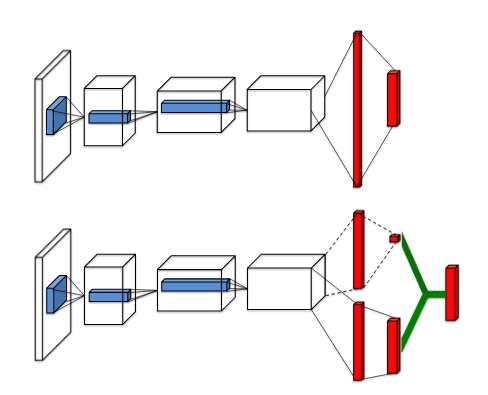
\includegraphics[width=0.3\textwidth]{images/duelingarch.png}
  \end{center}
  \caption{Dueling Architecture from original paper}
  \label{fig:duelingarch}
\end{wrapfigure}

The main idea is that it may not be always be important to know the value of every action given a state. The original paper explains this point well.

The only modification required is to the output of our network, where 
\begin{equation*}
    Q(s,a;\theta,\alpha,\beta) = V(s; \theta, \beta) + (A(s,a,;\theta,\alpha) - \frac{1}{|A|}\sum_{a'}\, A(s,a';\theta,\alpha))
\end{equation*}

\subsection{Prioritized Experience Replay}
Vanilla DQN uniformly samples from the experience replay buffer, which is not ideal since it may not always pick the most valuable information to learn from (i.e. largest TD error $\delta$).

PER solves this by assigning every sample with a priority value, $p$, where $p_i = |\delta_i| + \epsilon$, and the probability of picking sample $i$ is
\begin{equation*}
    P(i) = \frac{p_i^\alpha}{\sum_k p_k^\alpha}
\end{equation*}
To reduce bias caused by sampling high priority experiences more than lower priority ones, we use importance-sampling (IS) weights
\begin{equation*}
    w_i = (\frac{1}{N}\frac{1}{P(i)})^\beta
\end{equation*}
\section{Actor Critic Methods}
Policy gradient methods are low in bias, but it suffers from high variance since it cannot bootstrap.

Value-function approximation methods like DQN have lower variance (from bootstrapping), but as a result introduces bias.

Merging both of these, our critic learns a value function approximator, while our actor uses policy gradient to learn a stochastic policy, such that $\Delta\theta = \alpha \nabla_\theta\, log\, \pi_\theta (s,a)\, Q_w(s,a)$, where $Q_w(s,a)$ is provided by the critic
\subsection{Reducing variance with baseline}
To reduce variance of $Q_w(s,a)$, we subtract a baseline function, $B(s)$, from $Q_w(s,a)$. Note that $B(s)$ must not be a function of action (i.e. $B(s,a)$) so that our expectation does not change (i.e. $E_{\pi_\theta}[\nabla_\theta\,log\pi_\theta(s,a)(Q_w(s,a)-B_w(s)] \equiv E_{\pi_\theta}[\nabla_\theta\,log\pi_\theta(s,a)Q_w(s,a)]$.

A good baseline is the state value function $B(s)=V^\pi_\theta(s)$, such that $A^\pi_\theta(s,a) = Q^\pi_\theta(s,a) - V^\pi_\theta(s)$. Since $Q^\pi_\theta(s,a)=r+\gamma V(s')$, we realize that our advantage function can be our TD error $\delta$.

\section{Asynchronous Actor Critic Methods - A3C \& A2C}
Problems that A3C tries to solve:
\begin{itemize}
    \item Neural networks suffer from high variance, and as a result poor convergence, for online RL updates. This is due to strongly correlated data (i.e. frames from a video game).
    \item Experience replay buffers uses more memory and computation, and limits only to offline algorithms (where data can first be decorrelated).
\end{itemize}
Key ideas that A3C introduces:
\begin{itemize}
    \item Shared architecture between the actor and the critic
    \item Update on fixed-length segments of experience (n-step TD)
    \item Parallel worker threads, each with separate instances of the environment help decorrelate data
\end{itemize}

\subsection{Difference between A2C \& A3C}
The major difference between them is that for A3C, worker threads update the main, shared network in an asynchronous fashion, while A2C waits for all actors to complete their segments, before updating the main network, by taking the average over all actors.

A2C is shown to be able to utilize GPUs better (larger batch size), and prevents worker threads from using older versions of the main network.

\section{PPO - Proximal Policy Optimization}
\end{document}
